\subsection*{Problema 29}

\textbf{Enunciado:} Calcular la integral:\\
$\int \dfrac{dx}{\sin x - \cos x + 1}$

\textbf{Solución:}

Para resolver esta integral trigonométrica, aplicamos la sustitución universal de Weierstrass, definida como:

\begin{align*}
z &= \tan\left(\dfrac{x}{2}\right), \quad -\pi < x < \pi
\end{align*}

A partir de esta sustitución, las identidades trigonométricas fundamentales en términos de $z$ se expresan como:

\begin{align*}
\sin x &= \dfrac{2z}{1 + z^2}, \quad \cos x = \dfrac{1 - z^2}{1 + z^2} \\
dx &= \dfrac{2 \, dz}{1 + z^2}
\end{align*}

Sustituimos estas expresiones en la integral original del problema:

\begin{align*}
I &= \int \dfrac{\dfrac{2 \, dz}{1 + z^2}}{\dfrac{2z}{1 + z^2} - \dfrac{1 - z^2}{1 + z^2} + 1}
\end{align*}

Simplificamos el denominador encontrando un denominador común de $1 + z^2$:

\begin{align*}
I &= \int \dfrac{\dfrac{2 \, dz}{1 + z^2}}{\dfrac{2z - (1 - z^2) + (1 + z^2)}{1 + z^2}}
\end{align*}

Cancelamos el término $1 + z^2$ del denominador de ambas fracciones:

\begin{align*}
I &= \int \dfrac{2 \, dz}{2z - 1 + z^2 + 1 + z^2} \\
I &= \int \dfrac{2 \, dz}{2z^2 + 2z}
\end{align*}

Factorizamos el denominador y simplificamos la constante $2$:

\begin{align*}
I &= \int \dfrac{2 \, dz}{2(z^2 + z)} \\
I &= \int \dfrac{dz}{z(z + 1)}
\end{align*}

Aplicamos fracciones parciales al integrando:

\begin{align*}
\dfrac{1}{z(z + 1)} &= \dfrac{A}{z} + \dfrac{B}{z + 1} \\
1 &= A(z + 1) + Bz
\end{align*}

Evaluando en puntos clave para hallar $A$ y $B$:
Si $z = 0 \implies A = 1$.
Si $z = -1 \implies B = -1$.

Reescribimos la integral con las fracciones parciales:

\begin{align*}
I &= \int \left( \dfrac{1}{z} - \dfrac{1}{z + 1} \right) dz
\end{align*}

Integramos cada término de manera directa:

\begin{align*}
I &= \ln|z| - \ln|z + 1| + C \\
I &= \ln\left| \dfrac{z}{z + 1} \right| + C
\end{align*}

Regresamos a la variable original $x$ sustituyendo $z = \tan\left(\dfrac{x}{2}\right)$:

\begin{align*}
I &= \ln\left| \dfrac{\tan\left(\frac{x}{2}\right)}{\tan\left(\frac{x}{2}\right) + 1} \right| + C
\end{align*}

Resultado final de la integral indefinida:
\begin{align*}
\int \dfrac{dx}{\sin x - \cos x + 1} &= \ln\left| \dfrac{\tan\left(\frac{x}{2}\right)}{\tan\left(\frac{x}{2}\right) + 1} \right| + C
\end{align*}

\begin{figure}[H]
	\centering
	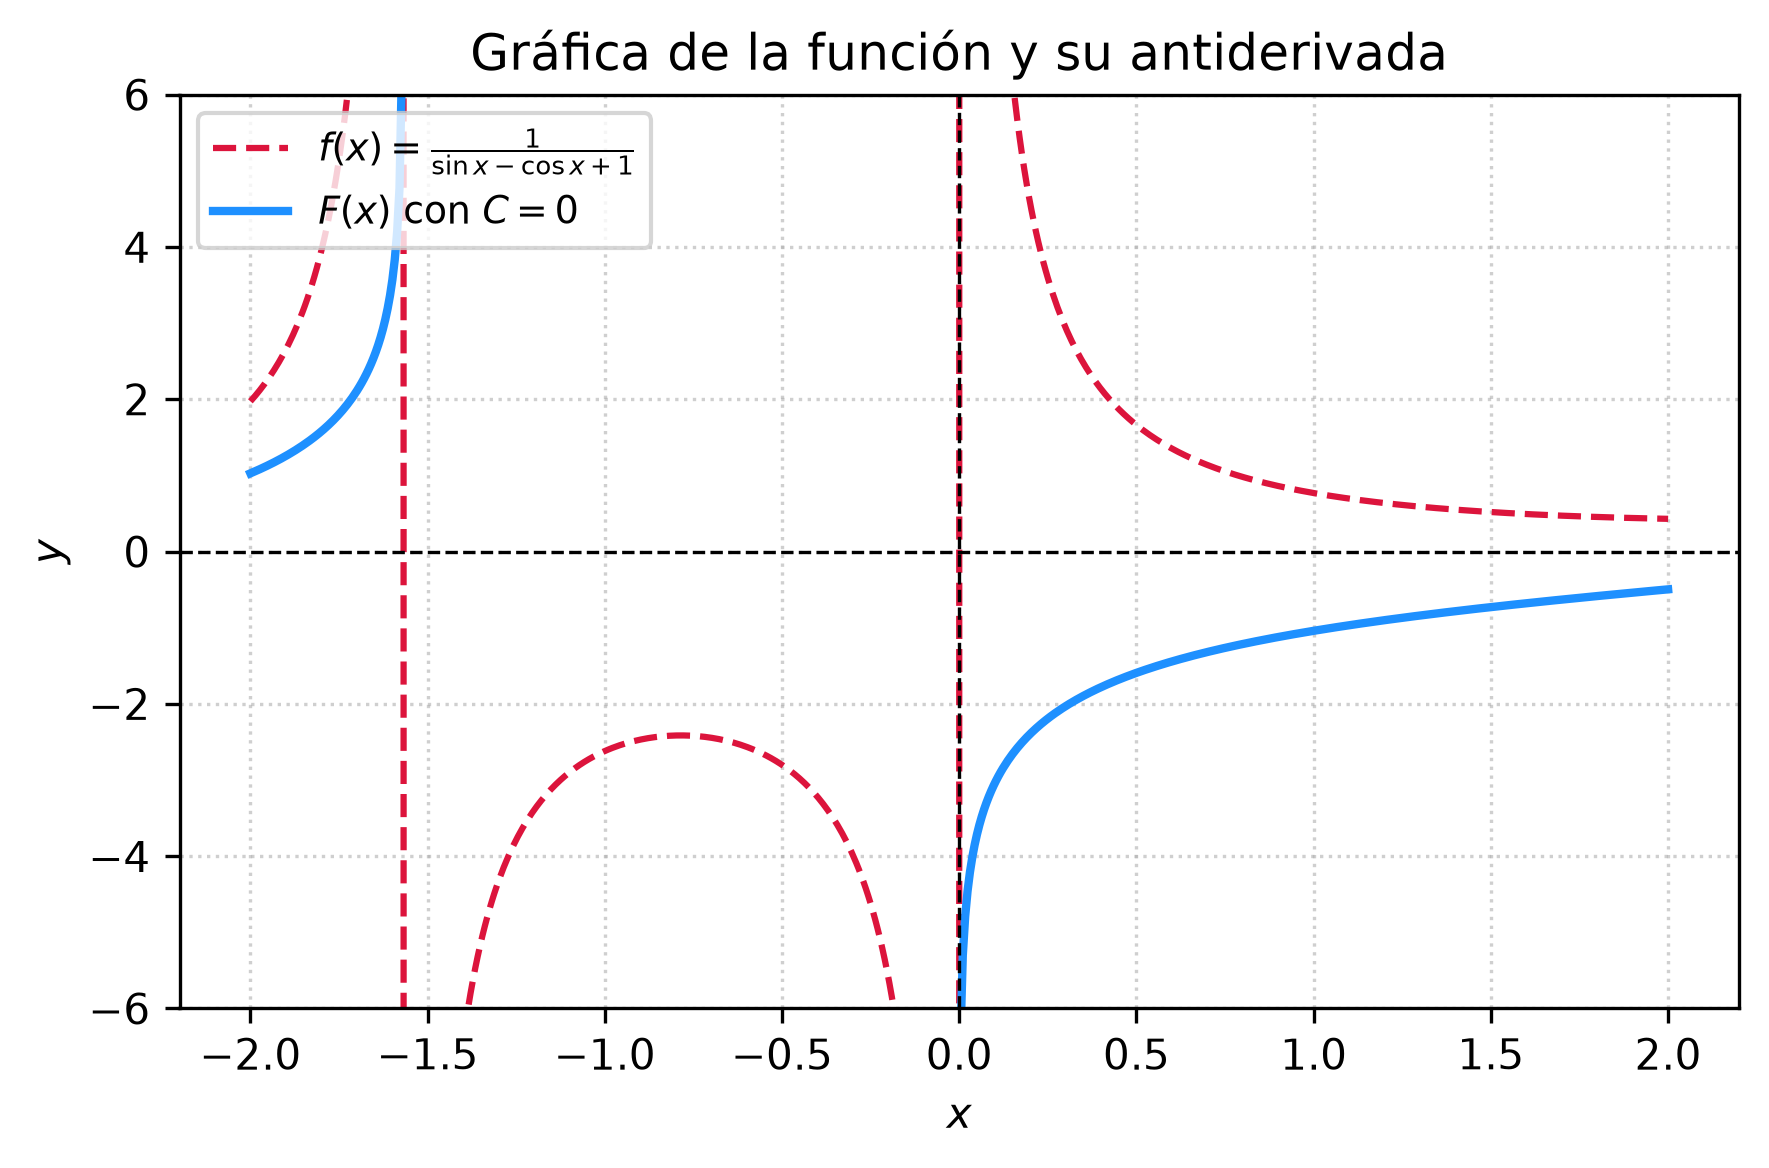
\includegraphics[width=\columnwidth]{semana_04/graficas/SEM04_P29_grafica.png}
	\caption{Representación gráfica de $f(x)$ y su antiderivada $F(x)$ evaluada para la constante de integración $C = 0$ (Problema 29).}
	\label{fig:problema29}
\end{figure}
